\section{Detekcija i opis značajki (engl. feature detection and description)}

\subsection{Odabir algoritma detekcije značajki}

Za uspješno prepoznavanje objekta potrebno je odabrati algoritam koji može detektirati značajke koje su invarijantne na promjene u okolini. U domeni detekcije značajki postoji nekoliko algoritama, koji se razlikuju po brzini i preciznosti detekcija. Primjerice SURF (eng. \textit{Speeded Up Robust Features}) dizajniran je kao brža aproksimacija SIFT-a, koristeći integralne slike s ubrzanje izračuna. ORB (eng. \textit{Oriented FAST and Rotated BRIEF}), koji kombinira brži detektor kutova FAST s binarnim deskriptorima BRIEF, što ga čini iznimno popularnim za uvjete mobilnih uređaja s ograničenim resursima. Unatoč manjoj brzini, u ovom radu se proučava i koristi SIFT, koji je razvio David Lowe~\cite{lowe2004sift}. Odluka se temelji na njegovoj preciznosti i robusnosti u odnosu na ostale algoritme, unatoč što zahtijeva više resursa. SIFT generira visokodimenzionalne deskriptore koji omogućuju pouzdanije prepoznavanje kompleksnih površina poput prirodne stijene. 

Iako su u modernom računalnom vidu pristupi temeljeni na dubokom učenju (eng. \textit{deep learning}) postali popularniji, njihova primjena u ovom problemu nije praktična radi količine potrebnih podataka za treniranje. U kontekstu ovog rada, to bi značilo da za svaki penjački smjer trebalo bi biti mnogo slika iz različitih kutova, udaljenosti i uvjeta osvjetljenja, te ih ručno kategorizirati. S obzirom da je sustav dinamičan i korisnici su oni koji dodaju penjačke smjerove, za svaki novi unos podatak potrebno bi bilo ponovno trenirati model. Takav proces prikupljanja podataka i treniranja modela je iznimno zahtjevan i nepraktičan. SIFT i drugi algoritmi detekcije značajki funkcioniraju na principu učenja iz jednog primjera, tj. potrebna je samo jedna referentna slika za kasnije prepoznavanje. 

\subsection{SIFT algoritam}

Rad SIFT algoritma može se podijeliti u četri faze. U prvoj fazi se detektiraju ekstremi u prostoru skale. Kako bi se postigla invarijantnost u skali, algoritam ne pretražuje značajke samo na originalnoj slici, već u trodimenzionalnom prostoru skale koji se generira postupnim zamućivanjem i skaliranjem originalne slike primjenom Gaussovih filtera s rastućom standardnom devijacijom. 
Cijeli proces se često provodi u oktavama, gdje se nakon određenog broja zamućenja slika smanjuje na pola veličine i proces se ponavlja. Time se dobivaju različite verzije slike, od oštre do zamućene, simulirajući pogled na objekt s različitih udaljenosti. Za efikasnu detekciju stabilnih točaka koje su neovisne o skali, SIFT koristi aproksimaciju Laplaceove-Gaussove funkcije zvanu razlika Gaussovih funkcija (eng. \textit{Difference of Gaussians, DoG}). DoG slike dobivaju se oduzimanjem dviju susjednih, različito zamućenih slika unutar iste oktave. Potencijalne ključne točke lociraju se kao lokalni minimum ili maksimum u DoG prostoru. Točka se smatra lokalnim ekstremom ako je njena vrijednost veća ili manja od svih osam susjednih piksela na istoj DoG slici, te svih 9 susjednih piksela na DoG slici iznad ili ispod nje - ukupno 26 susjeda.

Kandidati dobiveni u prethodnoj fazi trebaju se dalje filtrirati kako bi se odbacile nestabilne točke. Prvo se interpolira vrijednosti sub-piksela gdje se nalazi lokacija ekstrema. Ideja iza interpolacije je da se želi povećati preciznost i stabilnost ključnih točaka. Preciznije točke omogućuju bolje uparivanje te bolje naknadno korištenje značajnih točka, poput izračuna homografije. Nakon interpolacije primijenjuje se eliminacija točaka koje leže na rubovima. Rubovi su detektirani kao ekstremi, no točke na samom rubu su nepouzdane za precizno uparivanje jer je njihova lokacija duž samog ruba slabo definirana.

Kako bi se postigla invarijantnost na rotaciji, svakoj preostaloj ključnoj točki dodjeljuje se jedna ili više orijentacija. Orijentacija se izračunava na temelju lokalnog gradijenta slike u okolini ključne točke koristeći magnitudu i smjer gradijenta svakog piksela. Za svaku ključnu točku kreira se histogram orijentacija gradijenta s 36 spremnika koji svaki pokriva kut od 10 stupnjeva. 
Svaki unos u histogram uključuje u račun magnitudu gradijenta te udaljenost od centra ključne točke. Ako je piksel na oštroj kontrasnoj liniji magnituda gradijenta  biti če veća, također ako je piksel na rubu okoline, magnituda će biti manja i time utjecaj te orijentacije manji. Vrh tog histograma definira dominantnu orijentaciju ključne točke. Ako postoji više od jedne orijentacije, tj. ako postoji orijentacija koja je veća od 80\% od dominantne orijentacije, tada se kreira nova ključna točka sa istim položajem i skalom, ali s drugom orijentacijom. Time se povećava stabilnost uparivanja na mjestima s kompleksnim gradijentom.

Poslijednji korak je stvaranje jedistvenog numeričkog deskriptora za svaku ključnu točku. Oko ključne točke uzima se 16x16 piksela te se rotira u skladu s dominantnom orijentacijom čime se postiže nezavisnost rotacije. Rotirana okolina se zatim dijeli na 4x4 podregije. U svakoj podregiji računa se histogram orijentacija gradijenta s 8 spremnika i vrijednosti iz svih 16 histograma spaja se u jedan 128-dimenzionalni vektor te se vektor normalizira kako bi se smanjila ovisnost o osvjetljenju.

\begin{figure}[H]
    \centering
    \begin{subfigure}[b]{0.48\textwidth}
        \centering
        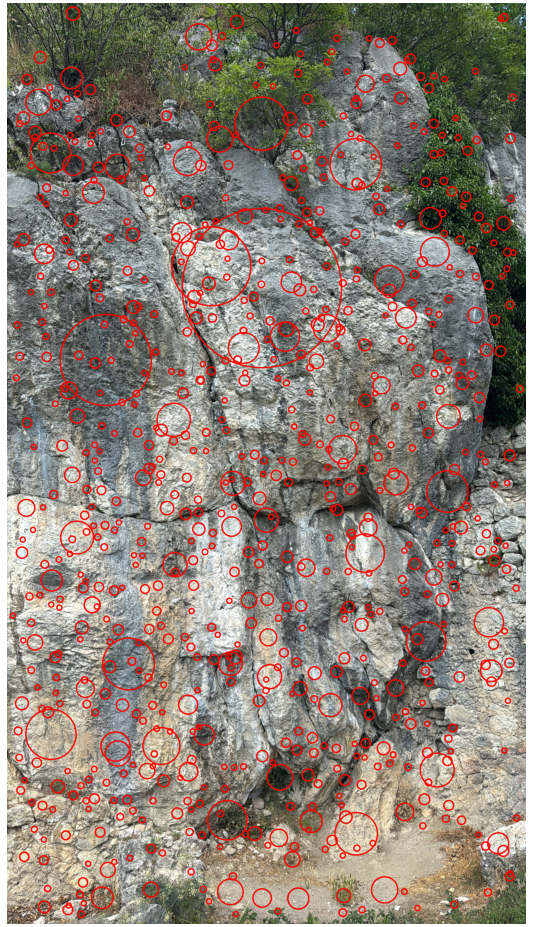
\includegraphics[width=\textwidth]{images/racunalniVid/feature_detection_train.png}
        \caption{Referentna slika penjačkog smjera}
        \label{fig:feature_detection_train}
    \end{subfigure}
    \hfill
    \begin{subfigure}[b]{0.48\textwidth}
        \centering
        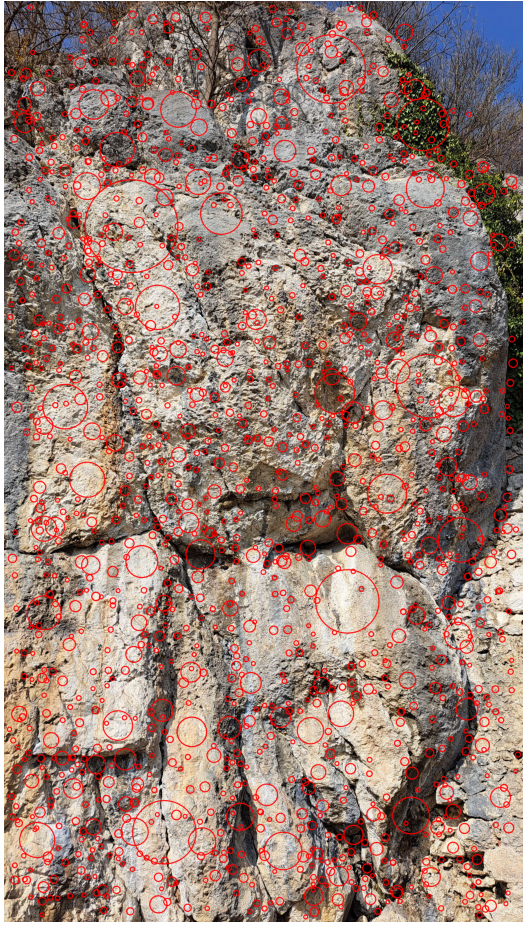
\includegraphics[width=\textwidth]{images/racunalniVid/feature_detection_frame.png}
        \caption{Slika s kamere mobilnog uređaja}
        \label{fig:feature_detection_frame}
    \end{subfigure}
    \caption{Detekcija značajki SIFT algoritmom}
    \label{fig:detekcija_znacajki}
\end{figure}

Izlaz iz SIFT algoritma je skup detektiranih značajki, tj. njen položaj, skala, orijentacija i 128-dimenzionalni deskriptor. Cijeli proces SIFT algoritma provodi se za refrentnu sliku penjačkog smjera te slike dobivene sa kamere mobilnog uređaja. Na slici~\ref{fig:detekcija_znacajki} prikazan je primjer detekcije značajki SIFT algoritmom za referentnu sliku penjačkog smjera i sliku dobivenu sa kamere mobilnog uređaja. Radi preglednosti prikazuju se samo značajke koje obuhvaćaju veću površinu.

